%%%%%%%%%%%%%%%%%%%%%%%%%%%%%%%%%%%%%%%%%%%%%%%%%%%%%
%%%%%%%%%%%%%%%%%%%%%%%%%%%%%%%%%%%%%%%%%%%%%%%%%%%%%
%\section{FCC work flow}
\section{Work flow}
\label{sec:fccworkflow}

%%%%%%%%%%%%%%%%%%%%%%%%%%%%%%%%%%%%%%%%%%%%%%%%%%%%%
\subsection{Monte-Carlo production}
\label{subsec:mcprod}

% /eos/experiment/fcc/helhc/utils/delphescards/helhc_v01/card.tcl
% /eos/experiment/fcc/hh/utils/delphescards/fcc_v02/muonMomentumResolutionVsP.tcl
Monte Carlo~(MC) simulated event samples were used to simulate the response of the DELPHES detector to signal and backgrounds. The muon momentum resolution is assumed to be $\sigma(p)/p \approx 6\%~(10\%)$ at $\pt= 20~(5)$ TeV and $|\eta| \approx 0.$ for FCC-hh (HE-LHC) scenario. Signals are generated with {\scshape Pythia}~8.230 ($p8$)~\cite{Sjostrand:2014zea} using the leading order cross-section from the generator.
All lepton flavour decays of the $\ZpSSM$ are generated assuming universality of the couplings.
The SM backgrounds are Drell-Yan, di-jet (QCD), top pairs (\ttbar), $VV$ and \vj\ where $V=W/Z$, which were generated using {\scshape MG5\_}a{\scshape MC@NLO}~2.5.2 ($mg$)~\cite{Alwall:2014hca} at leading order only. A k-factor of 2 is applied to all the background processes. \newline
{\scshape Pythia} independent samples have been produced for Multi-Variate taggers training (section~\ref{subsec:mvatagger}). QCD has been produced to avoid useless events thanks to a filtering chosen to ensure to have consistent leading jet $\pT$ as the signals considered (pTHatMin = 2500, bias2Selection = on, bias2SelectionPow = 6).\newline
Tables~\ref{tab:MCtable_bkgd} and ~\ref{tab:MCtable_sig} are summarising all the background and signal samples produced for the various analysis presented in this document.

\begin{table}[!htb]\centering
\begin{tabular}{|c|c|c|c|}
\hline
\hline		
process & Ngen & generator & k-factor \\
\hline		
pp\_$ee$\_5f\_HT & $\sim$5M & $mg+p8$ & 2 \\
pp\_$\mu\mu$\_5f\_HT & $\sim$5M & $mg+p8$ & 2 \\
pp\_$\tau\tau$\_5f\_HT & $\sim$5M & $mg+p8$ & 2 \\
pp\_$jj$\_5f\_HT ($j$ = $u$, $d$, $c$, $s$ or $b$) & $\sim$5M & $mg+p8$ & 2 \\
pp\_$tt$\_5f\_HT & $\sim$5M & $mg+p8$ & 2 \\
pp\_$Vj$\_5f\_HT ($V$ = $W$ or $Z$ and $j$ = $u$, $d$, $c$, $s$ or $b$) & $\sim$5M & $mg+p8$ & 2 \\
pp\_$VV$\_5f\_HT ($V$ = $W$ or $Z$) & $\sim$5M & $mg+p8$ & 2 \\
\hline
\hline
\end{tabular}
\caption{Summary of generated background samples. The following HT (scalar sum of all visible paticles momentum at generator level) binnings have been used : [500, 1000], [1000, 2000], [2000, 5000], [5000, 10000], [10000, 27000], and [27000, 100000] GeV. 5f stands for flavour quaks : u, d, c ,s  and b.}
\label{tab:MCtable_bkgd}
\end{table}

\begin{table}[!htb]\centering
\begin{tabular}{|c|c|c|c|}
\hline
\hline		
process & Ngen & generator & k-factor \\
\hline		
pp\_$Z'_{SSM}$\_$ll$ ($l$ = $e$, $\mu$ or $\tau$) & \multirow{2}{*}{$\sim$1M} & \multirow{2}{*}{$p8$} & \multirow{2}{*}{1} \\
mass : \{2,4,5,6,8,10,12,14,15,16,18,20,25,30,35,40,45,50\} TeV & & & \\
\hline		
pp\_$Z'_{flavano}$\_$\mu\mu$\_5f & \multirow{2}{*}{$\sim$1M} & \multirow{2}{*}{$mg+p8$} & \multirow{2}{*}{1} \\
mass : \{4,6,8,10,12,14,15,16,18,20,25,30,35,40,45\} TeV & & & \\
\hline		
pp\_$LQ$\_$\mu\mu$\_5f & \multirow{2}{*}{$\sim$1M} & \multirow{2}{*}{$mg+p8$} & \multirow{2}{*}{1} \\
mass : \{4,6,8,10,12,14,16,18,20,22,24,26,28,30,32,34,36,38,40\} TeV & & & \\
\hline		
pp\_$Z'_{TC2}$\_$tt$ & \multirow{2}{*}{$\sim$1M} & \multirow{2}{*}{$p8$} & \multirow{2}{*}{1} \\
mass : \{2,5,10,15,20,25,30,35\} TeV & & & \\
\hline		
pp\_$RSG$\_$WW$ & \multirow{2}{*}{$\sim$1M} & \multirow{2}{*}{$p8$} & \multirow{2}{*}{1} \\
mass : \{2,5,10,15,20,25,30,35\} TeV & & & \\
\hline		
pp\_$Q^*$\_$qq$ ($q$ = $u$, $d$, $c$, $s$, $b$ or $t$) & \multirow{2}{*}{$\sim$0.6M} & \multirow{2}{*}{$p8$} & \multirow{2}{*}{1} \\
mass : \{15,20,25,30,35,40,45,50\} TeV & & & \\
\hline		
pp\_$Z'_{SSM}$\_$jj$ ($j$ = $u$, $d$, $c$, $s$ or $b$) & \multirow{2}{*}{$\sim$1.2M} & \multirow{2}{*}{$p8$} & \multirow{2}{*}{1} \\
mass : \{10,15,20,25,30,35,40,45,50\} TeV & & & \\
\hline
\hline
\end{tabular}
\caption{Summary of generated signal samples.}
\label{tab:MCtable_sig}
\end{table}

%%%%%%%%%%%%%%%%%%%%%%%%%%%%%%%%%%%%%%%%%%%%%%%%%%%%%%%%%%%%%%%%%%%%%%%%%%%%%%%%%%%%%%%%%%%%
\subsection{Detector parameterizations}
\label{subsec:detparam}

The FCC study group is using the Delphes software package to emulate the response a detector. 
For the FCC one the baseline parameters are: TBD
We also consider two variations around it as well as the CMS configuration.
Talk about how we use this same detector for HE-LHC with only energy change.


%%%%%%%%%%%%%%%%%%%%%%%%%%%%%%%%%%%%%%%%%%%%%%%%%%%%%
\subsection{Multi-Variate based selection}
\label{subsec:mvatagger}

% from physics paper
An important ingredient of the \Zptt\ and \rsg\ searches is the identification of heavy boosted top quarks and $W$ bosons. Two jet taggers using Boosted Decision Trees (BDT) were developed to discriminate $W$ and top jets against the $\pt$ di-jet background.
\newline
The BDT parameters used are the following : NTrees=600, MaxDepth=4, AdaBoost, AdaBoostBeta=0.15, SeparationType=GiniIndex, nCuts=100, PruneMethod=NoPruning. As the tagger goal is to discriminate jets, a jet collection is build to feed the BDT and a simple event selection is applied by requiring only events without isolated leptons.
The input variables are defined to be the same as the ones used to perform cut-based associated analysis (\Zptt\ and \rsg\ in section~\ref{subsec:hadreso}) and the idea is to fully exploit these informations thanks to the BDT. Summary of samples used to train the BDT, the statistics of the input jet samples and variables (ordered by training weight) can be found in table~\ref{tab:TMVA_summary}.
\newline
Top and $W$ taggers were optimised using jets with a transverse boost of $\pt=$10 TeV. At these extreme energies, $W$ and top jets have a characteristic angular size $R=0.01-0.02$, i.e smaller than the typical electromagnetic and hadronic calorimeter cells. Following the approach described in~\cite{Larkoski:2015yqa}, we exploit the superior track angular resolution and reconstruct jets from tracks only (track jets) using the anti-$k_T$ algorithm with a parameter R=0.2. The missing neutral energy is corrected for by rescaling the track 4-momenta by the factor $\ptSup{trk}/\ptSup{PF}$, where $\ptSup{trk}$ is the track Jet \pt\ and $\ptSup{PF}$ is the Particle-Flow Jet \pT. In what follows, we will simply refer to ``track jets'' as the jet collection that includes the aforementioned rescaling.
\newline
The boosted top tagger is built from jet substructure observables: the soft-dropped jet mass~\cite{Larkoski:2014wba} and N-subjettiness~\cite{Thaler:2010tr} variables $\tau_{1,2,3}$ and their ratios $\tau_{2}/\tau_{1}$ ($\tau_{21}$) and $\tau_{3}/\tau_{2}$ ($\tau_{32}$). The $W$-jet versus QCD-jet tagger also uses an ``isolation-like'' variable that exploits the absence of high \pt\ final state-radiation (FSR) in the vicinity of the $W$ decay products. We call these variables $E_{F}(n,\alpha)$ and define them as:

\begin{equation}
E_{F}(n,\alpha) =  \frac{\sum \limits_{\frac{n-1}{5}\alpha < \Delta R(k,jet)< \frac{n}{5}\alpha} \ptSup{(k)}}{\sum \limits_{\Delta R(k,jet)< \alpha} \ptSup{(k)}}
\end{equation}
\newline
We use $\alpha=0.05$. We construct 5 variables $E_{F}(n,\alpha)$ with $n=1..5$ and provide them as input to the BDT. The $E_{F}(1,0.05)$ observable is shown in 
%Figure~\ref{figure:hadronicresonances:BDTeff} (left).
Figures~\ref{fig:TMVA_final_result} (left) and~\ref{fig:TMVA_inputs_w}.
%The final performance of the $W$ and top tagger is shown in Figure~\ref{figure:hadronicresonances:BDTeff} (right).
The final performance of the $W$ and top tagger is shown in Figure~\ref{fig:TMVA_final_result} (right). More $TMVA$ (Toolkit for Multivariate Data Analysis) detailed results can be found in appendix~\ref{appendix:tmva}.
The $W$ tagging performance has significantly better performance due to the use of the energy-flow variables. We choose our working points with a top and $W$ tagging efficiencies of $\epsilon_S^{\text{top}}=60\%$ and $\epsilon_S^{\text{W}}=90\%$ corresponding respectively to a background efficiency of $\epsilon_B^{\text{top}}=\epsilon_B^{\text{W}}=10\%$. These working points corresponds to a cut at 0.15 on the BDT output value for both taggers.
\newline
Some extra cross-checks have been performed. First, removing fully correlated variables have been tried and it doesn't change anything to performances obtained. Then the BDT response has been shown for different signal masses to understand how much the analyses can be mass dependent (Figure \ref{fig:BDT_signal_shape_comparison}). From the cuts defined in the analysis level at 0.15, the BDT shape response difference is not changing so much the proportion of signal kept and it removes 90\% and 95\% of QCD for thad and Whad taggers respectively.

\begin{table}[!htb]\centering
\begin{tabular}{|c|c|c|}
\hline
\hline			
 & Whad/QCD & thad/QCD \\
\hline                        
%\hline                        
Sample signal     & pp\_$RSG$\_$WW$\_20TeV (1M) & pp\_$Z'_{TC2}$\_$tt$\_20TeV (1M) \\
Sample background & pp\_$jj$\_lo ($j$ = $u$, $d$, $c$, $s$ or $b$) (920k) & pp\_$jj$\_lo ($j$ = $u$, $d$, $c$, $s$ or $b$) (920k)               \\
\hline
Train stat. signal (jets)     & 1117500 & 1432192 \\
Train stat. background (jets) & 1578098 & 1578098 \\
\hline
% rename them
ranked variables & $Jet^{trk02}(\tau_3)$ (0.12)      & $Jet^{trk02}(\tau_1)$ (0.21) \\
(ordered)        & $Jet^{trk02}(M^{SD Corr})$ (0.11) & $Jet^{trk02}(M^{SD Corr})$ (0.17) \\
                 & $Jet^{trk02}(\tau_{31})$ (0.10)   & $Jet^{trk02}(\tau_{31})$ (0.11) \\
                 & $Jet(Flow55)$ (0.09)              & $Jet^{trk02}(\tau_2)$ (0.10) \\
                 & $Jet(Flow45)$ (0.09)              & $Jet^{trk02}(\tau_3)$ (0.09) \\
                 & $Jet(Flow15)$ (0.08)              & $Jet^{trk08}(M^{SD Corr})$ (0.09) \\
                 & $Jet(Flow25)$ (0.07)              & $Jet^{trk04}(M^{SD Corr})$ (0.09) \\
                 & $Jet(Flow35)$ (0.06)              & $Jet^{trk02}(\tau_{32})$ (0.08) \\
                 & $Jet^{trk02}(\tau_{21})$ (0.06)   & $Jet^{trk02}(\tau_{21})$ (0.06) \\
                 & $Jet^{trk08}(M^{SD Corr})$ (0.06) &  \\
                 & $Jet^{trk04}(M^{SD Corr})$ (0.06) &  \\
                 & $Jet^{trk02}(\tau_1)$ (0.05)      &  \\
                 & $Jet^{trk02}(\tau_2)$ (0.04)      &  \\
                 & $Jet^{trk02}(\tau_{32}$ (0.02)    &  \\
\hline
\hline
\end{tabular}
\caption{Summary of BDT informations used to train Whad/thad VS QCD taggers.}
\label{tab:TMVA_summary}
\end{table}

\begin{figure}[!htbp]\centering
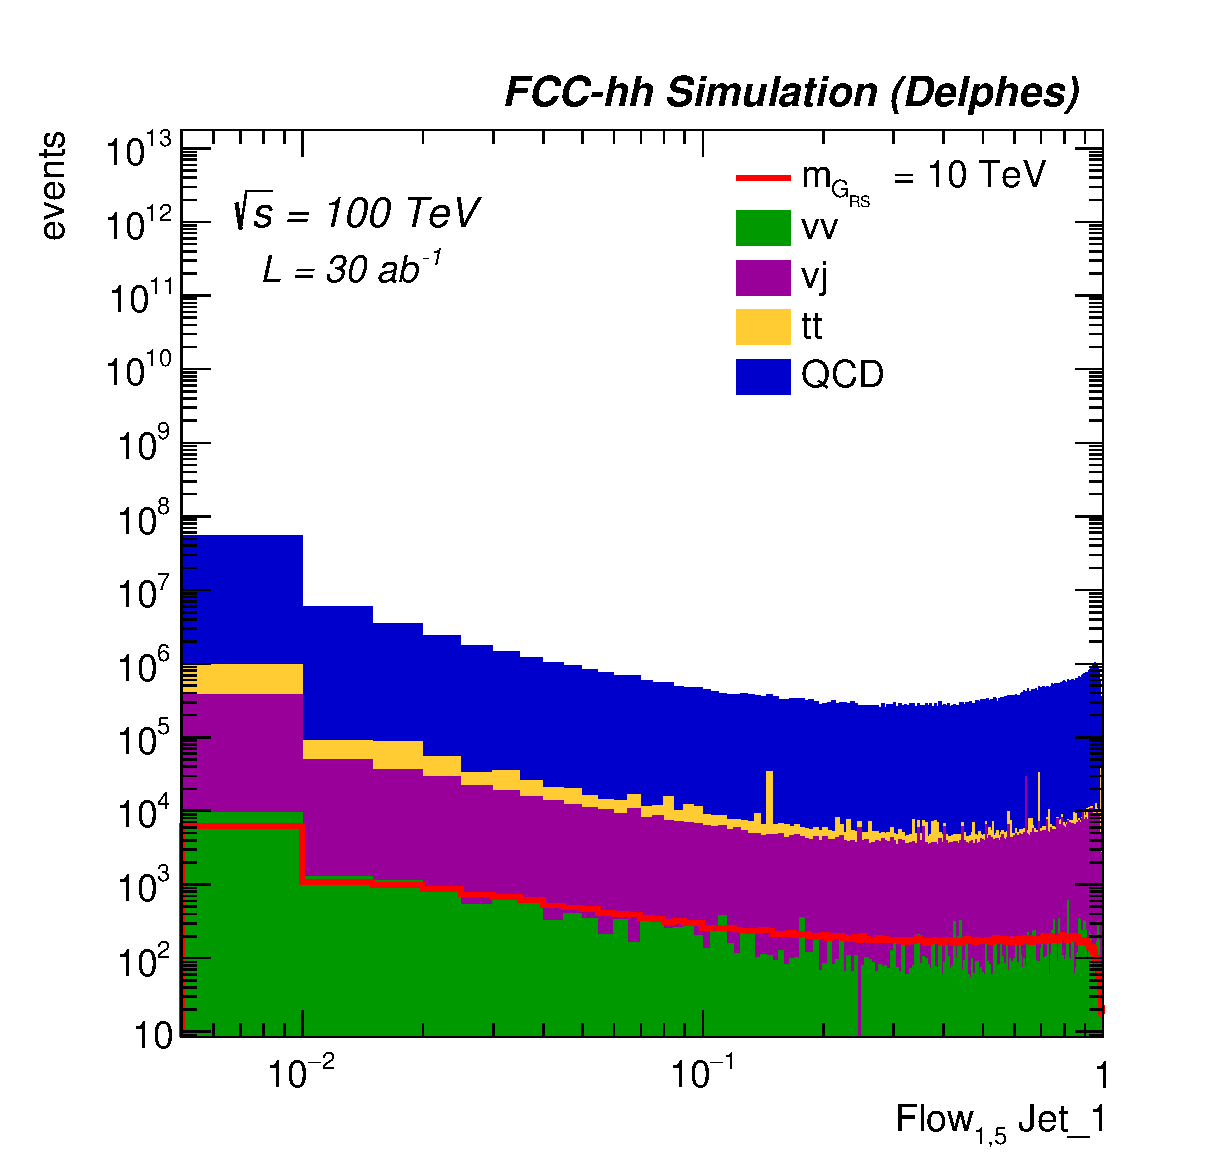
\includegraphics[width=0.33\textwidth]{Fig/TMVA/Jet1_Flow15_sel0_nostack_logx.eps}
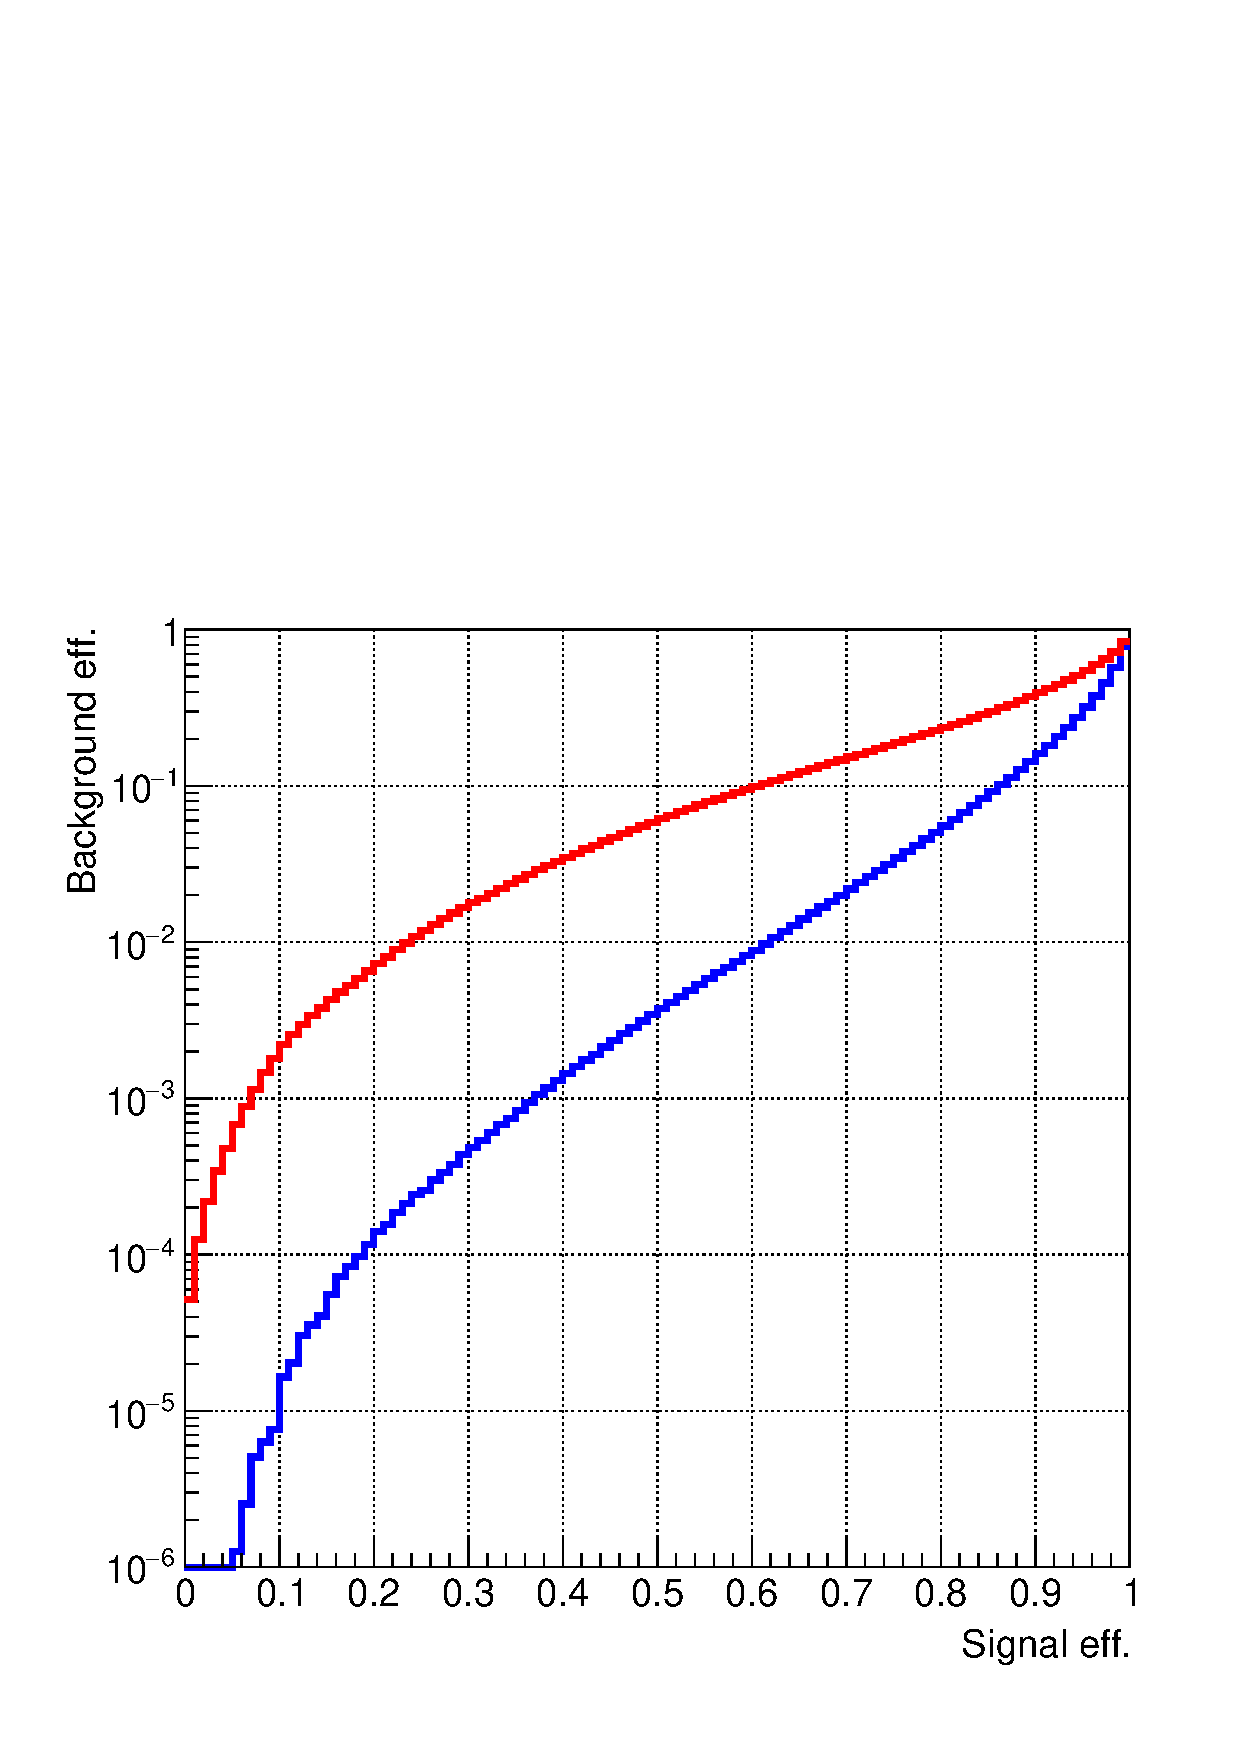
\includegraphics[width=0.33\textwidth,trim={0 0.5cm 0 0},clip]{Fig/TMVA/effQCD_vs_effWhadBlue_thadRed_log.pdf}
\caption{Left: Energy-flow ($E_{F}(1,0.05)$) observable for W and QCD jets. Right: Di-jet rejection versus signal efficiency for the two taggers, W in blue and top in red.}
\label{fig:TMVA_final_result}
\end{figure}

%\clearpage
%\newpage

%%%%%%%%%%%%%%%%%%%%%%%%%%%%%%%%%%%%%%%%%%%%%%%%%%%%%
\subsection{Tag Rate Function}
\label{subsec:trf}
The modeling of the backgrounds in the high tagging regimes is a challenging task. 
The requirement of $b$ tagging in some MC samples can drastically reduce the available statistics.
This shortage of events that pass the $b$-tagging cut in the signal regime, in conjunction with the large cross section of some of the backgrounds can lead to very spiky templates. 
\newline
To overcome this problem the tag rate function (TRF) method is introduced. 
By using the TRF method, no event is cut based on its $b$-tagging count, but instead all the events are weighted.
This weight can be interpreted as the probability of the given event to contain the desired number of $b$ jets. 
To achieve this, the tagging efficiency (a function of $\eta$, $\pt$ and true jet flavour) was
used to calculate the event weight based on the kinematics and flavour of the jets found in each event.
\newline
Given a jet with $\eta$, $\pt$ and flavour $f$, its tagging probability can be noted as:
\begin{equation*}
	\varepsilon \left(f,|\eta|,\pt\right)
\end{equation*}
\newline
For a given event with $N$ jets, its probability of containing exactly one $b$-tag jet can be computed as:
\begin{equation*}
	P_{=1} = \sum\limits_{i=1}^N \left( \varepsilon_{i} \prod\limits_{i \neq j} \left( 1 - \varepsilon_{j} \right) \right)
\end{equation*}
\newline
In the same way, it can be used to compute the probability for inclusive $b$-tag selections:
\begin{align*}
	P_{=0} &= \prod\limits_{i=1}^N \left( 1 - \varepsilon_{j} \right) \\
	P_{\geq 1} &= 1 - P_{=0}
\end{align*}
\newline
It was verify that the TRF methods agrees well with the direct tagging.

%%%%%%%%%%%%%%%%%%%%%%%%%%%%%%%%%%%%%%%%%%%%%%%%%%%%%
\subsection{Mass spectrum fit}
Despite the fact that very large amount of Monte-Carlo statistic has been simulated in bins of $\hht$
and the usage of techniques to save events with TRF methods,
there are still large statistical fluctuations from high weight events.
In order to reduce this effect, a function is used to fit the background distribution,
\begin{equation}
f(z)=p_1(1-z)^{p_2}z^{p_3}z^{p_{4}logz}
\end{equation}
where $z=m_{jj}/\sqrt{s}$. This fit is used in order to have a smooth shape for the backgrounds, while the normalisation is taken prior to the fit (see figure~\ref{fig:hadronicresonances_nofit}).

\begin{figure}[!htb]\centering
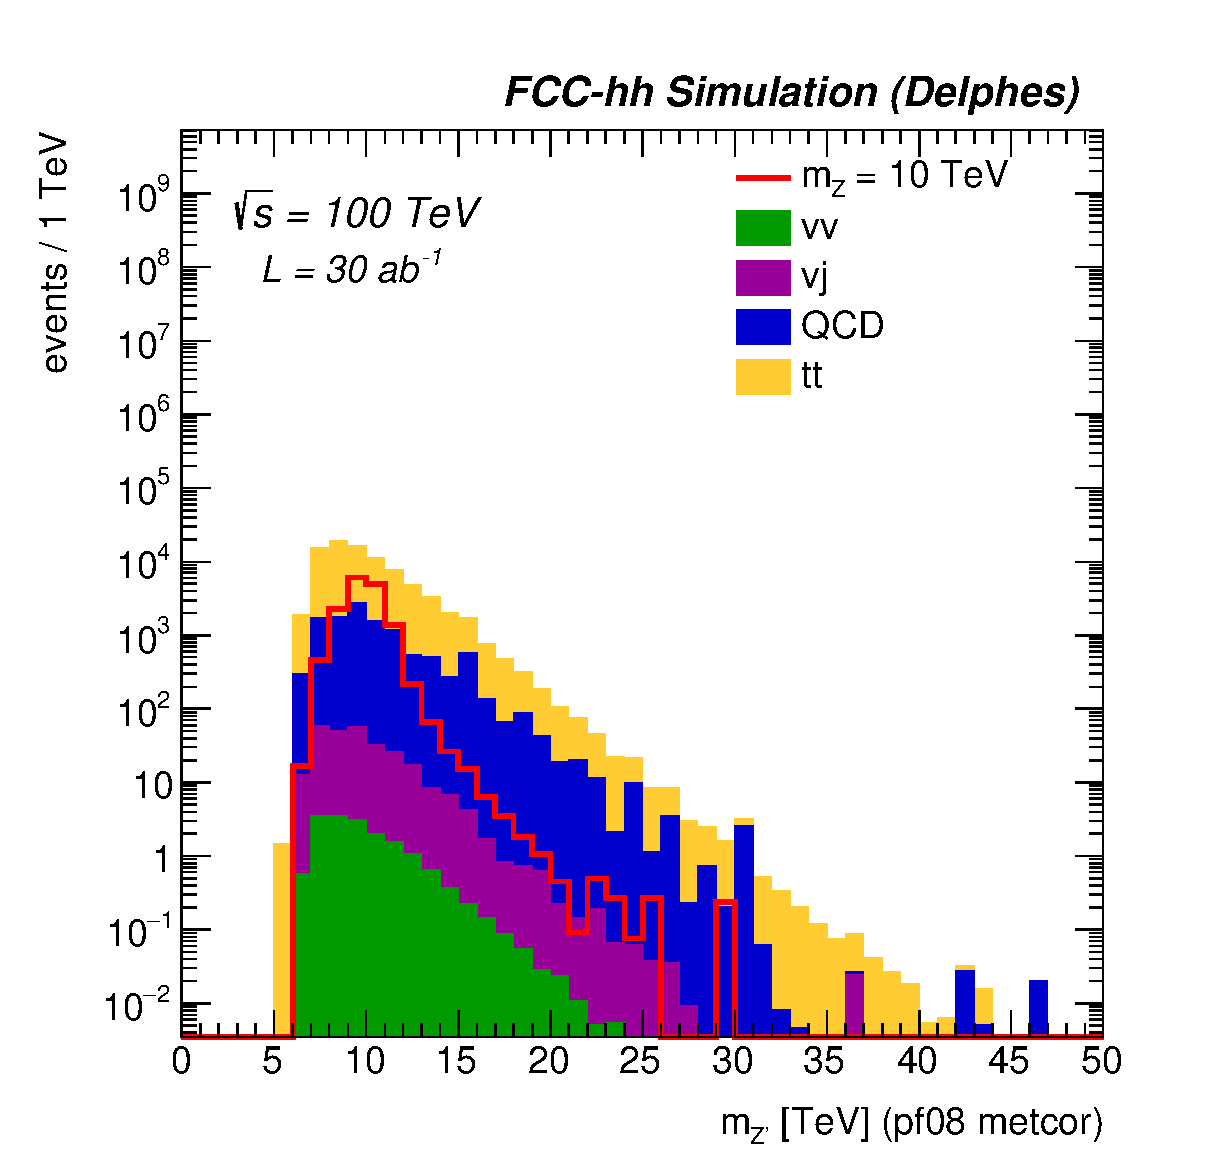
\includegraphics[width=0.33\columnwidth]{Fig/Zptt/Mj1j2_pf08_MetCorr_sel8_nostack_log.eps}
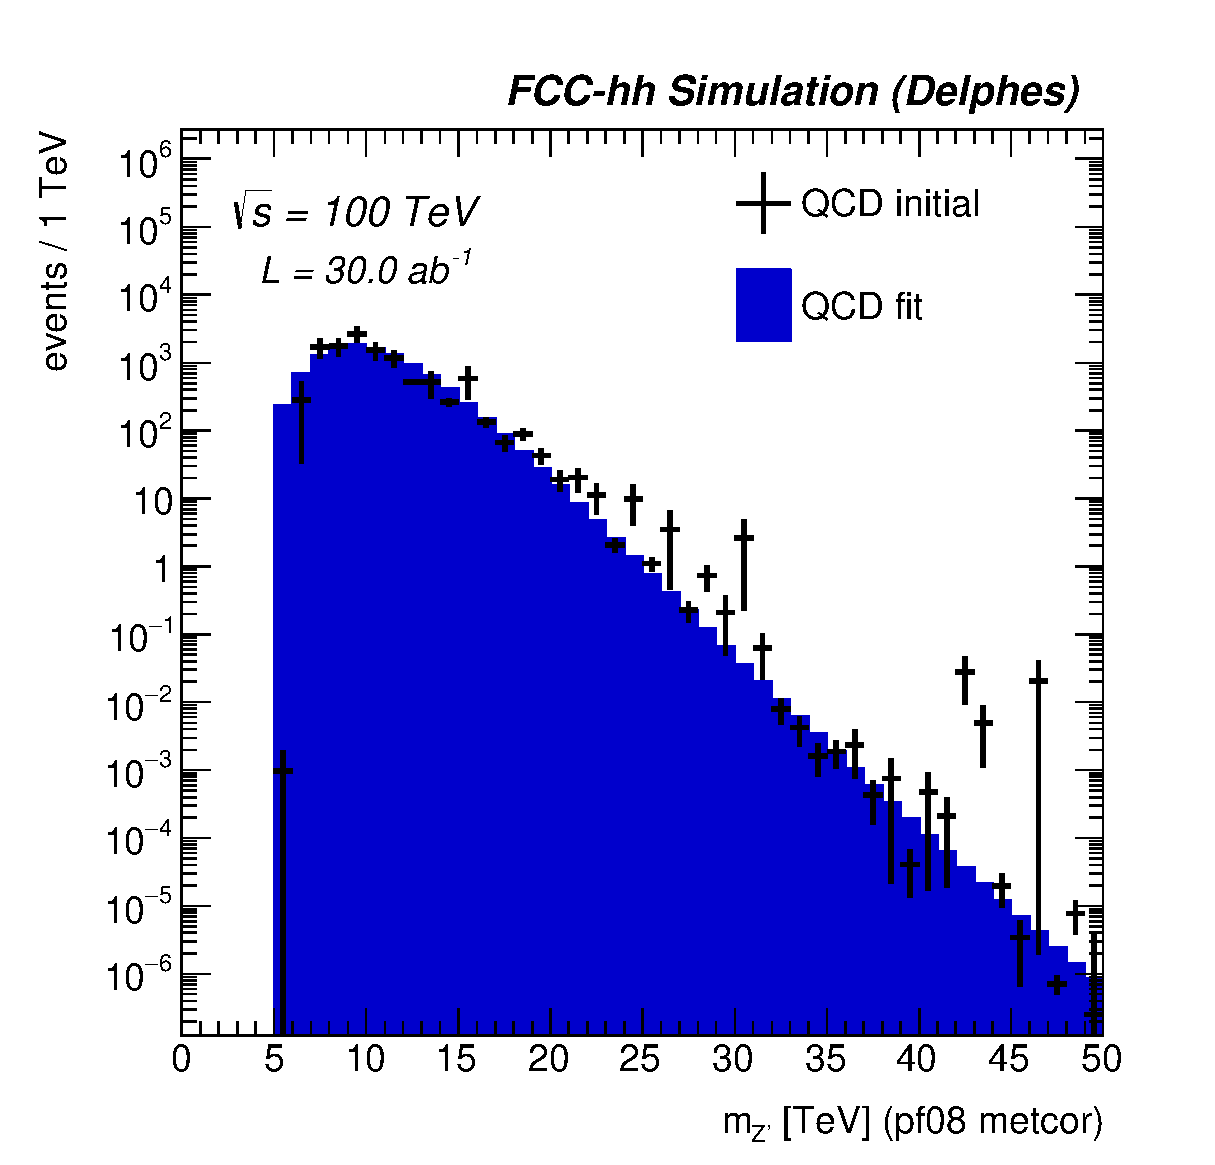
\includegraphics[width=0.33\columnwidth]{Fig/Zptt/Zptt_QCD_sel8_Mj1j2_pf08_MetCorr_fit.eps}
\caption{Invariant mass prior to fit.}
\label{fig:hadronicresonances_nofit}
\end{figure}

%%%%%%%%%%%%%%%%%%%%%%%%%%%%%%%%%%%%%%%%%%%%%%%%%%%%%
\subsection{Limit settings}
\label{subsec:limitsettings}

Develop here ?
